\documentclass{article}
\usepackage{tikz, comment}
\usepackage{pifont}
\usepackage{fontspec}
\usetikzlibrary{arrows, decorations.markings, decorations.pathreplacing}
\begin{comment}
:Title: Not defined yet
:Tags: pi;;sine, sin ;area using polar coordinates, polar integral formula ;moment;polar form of a complex number
:Prob: 0.4135;0.3766;0.3631;0.3572;0.348
:Slug: No name yet

Description Here.........
\end{comment}
\begin{document}\centering

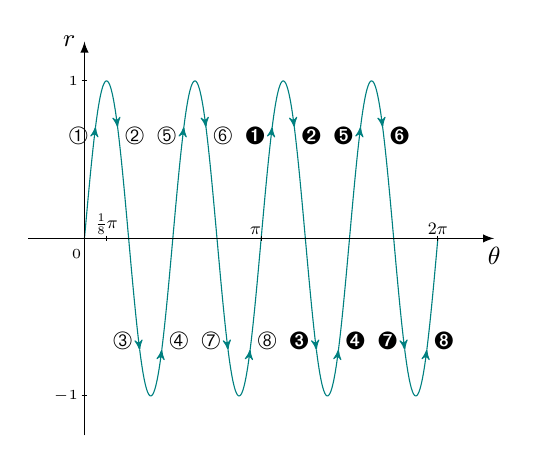
\begin{tikzpicture}[>=latex,xscale=.5/0.7, yscale=.5*4][font=\sf\small]

\draw[->, >=stealth', teal, samples=100, smooth, domain=0:pi/16, variable=\t]
plot ({\t}, {sin(4*\t r)}) -- ({pi/16}, {sin(4*(pi/16) r)});

\foreach \n in {1,3,...,29}
\draw[->, >=stealth', teal, samples=100, smooth, domain=(\n)*pi/16:(\n+2)*pi/16, variable=\t]
plot ({\t}, {sin(4*\t r)}) -- ({(\n+2)*pi/16}, {sin(4*((\n+2)*pi/16) r)});

\draw[teal, samples=150, smooth, domain=31*pi/16:2*pi, variable=\t]
plot ({\t}, {sin(4*\t r)});

%\draw[xstep=1cm,ystep=1cm,color=gray!80] (0, -1) grid (8, 8);
\foreach \x in {}
\draw (\x,2pt/6) -- (\x,-2pt/6)
node[anchor=north] {\tiny$\x$}
;
\draw ({1*pi/8},2pt/4) -- ({1*pi/8},-2pt/4)node[anchor=south, xshift=0, scale=0.7] {$\frac{1}{8}\pi$};
\draw ({pi},2pt/4) -- ({pi},-2pt/4)node[anchor= south, xshift=-2, scale=0.7] {$\pi$};
\draw ({2*pi},2pt/4) -- ({2*pi},-2pt/4)node[anchor= south, xshift=0, scale=0.7] {$2\pi$};

\foreach \x in {}
\draw (\x,2pt/2.5) -- (\x,-2pt/2.5)
node[anchor=south] {\tiny$\x$}
;
\foreach \y in {-1,1}
\draw (-2pt*0.7,\y) -- (2pt*0.7,\y)
node[anchor=east] {\tiny $\y$}
;

\draw[->] (-1, 0) -- ({2*pi+1}, 0)node[below] {\small $\theta$} ;
\draw[->] (0, {-2.5/2}) -- (0, {2.5/2})node[left] {\small $r$} ;

\node at ({pi/8-0.5}, {1.3/2}) {\ding{192}};
\node at ({pi/8+0.5}, {1.3/2}) {\ding{193}};
\node at ({3*pi/8-0.5}, {-1.3/2}) {\ding{194}};
\node at ({3*pi/8+0.5}, {-1.3/2}) {\ding{195}};

\node at ({5*pi/8-0.5}, {1.3/2}) {\ding{196}};
\node at ({5*pi/8+0.5}, {1.3/2}) {\ding{197}};
\node at ({7*pi/8-0.5}, {-1.3/2}) {\ding{198}};
\node at ({7*pi/8+0.5}, {-1.3/2}) {\ding{199}};

\node at ({9*pi/8-0.5}, {1.3/2}) {\ding{202}};
\node at ({9*pi/8+0.5}, {1.3/2}) {\ding{203}};
\node at ({11*pi/8-0.5}, {-1.3/2}) {\ding{204}};
\node at ({11*pi/8+0.5}, {-1.3/2}) {\ding{205}};

\node at ({13*pi/8-0.5}, {1.3/2}) {\ding{206}};
\node at ({13*pi/8+0.5}, {1.3/2}) {\ding{207}};
\node at ({15*pi/8-0.5}, {-1.3/2}) {\ding{208}};
\node at ({15*pi/8+0.5}, {-1.3/2}) {\ding{209}};

\node at (-0.2*0.7, -0.2/2) {\tiny$0$};

\end{tikzpicture}\hskip0.5cm
\end{document}